% Options for packages loaded elsewhere
\PassOptionsToPackage{unicode}{hyperref}
\PassOptionsToPackage{hyphens}{url}
%
\documentclass[
]{article}
\usepackage{amsmath,amssymb}
\usepackage{iftex}
\ifPDFTeX
  \usepackage[T1]{fontenc}
  \usepackage[utf8]{inputenc}
  \usepackage{textcomp} % provide euro and other symbols
\else % if luatex or xetex
  \usepackage{unicode-math} % this also loads fontspec
  \defaultfontfeatures{Scale=MatchLowercase}
  \defaultfontfeatures[\rmfamily]{Ligatures=TeX,Scale=1}
\fi
\usepackage{lmodern}
\ifPDFTeX\else
  % xetex/luatex font selection
\fi
% Use upquote if available, for straight quotes in verbatim environments
\IfFileExists{upquote.sty}{\usepackage{upquote}}{}
\IfFileExists{microtype.sty}{% use microtype if available
  \usepackage[]{microtype}
  \UseMicrotypeSet[protrusion]{basicmath} % disable protrusion for tt fonts
}{}
\makeatletter
\@ifundefined{KOMAClassName}{% if non-KOMA class
  \IfFileExists{parskip.sty}{%
    \usepackage{parskip}
  }{% else
    \setlength{\parindent}{0pt}
    \setlength{\parskip}{6pt plus 2pt minus 1pt}}
}{% if KOMA class
  \KOMAoptions{parskip=half}}
\makeatother
\usepackage{xcolor}
\usepackage[margin=1in]{geometry}
\usepackage{color}
\usepackage{fancyvrb}
\newcommand{\VerbBar}{|}
\newcommand{\VERB}{\Verb[commandchars=\\\{\}]}
\DefineVerbatimEnvironment{Highlighting}{Verbatim}{commandchars=\\\{\}}
% Add ',fontsize=\small' for more characters per line
\usepackage{framed}
\definecolor{shadecolor}{RGB}{248,248,248}
\newenvironment{Shaded}{\begin{snugshade}}{\end{snugshade}}
\newcommand{\AlertTok}[1]{\textcolor[rgb]{0.94,0.16,0.16}{#1}}
\newcommand{\AnnotationTok}[1]{\textcolor[rgb]{0.56,0.35,0.01}{\textbf{\textit{#1}}}}
\newcommand{\AttributeTok}[1]{\textcolor[rgb]{0.13,0.29,0.53}{#1}}
\newcommand{\BaseNTok}[1]{\textcolor[rgb]{0.00,0.00,0.81}{#1}}
\newcommand{\BuiltInTok}[1]{#1}
\newcommand{\CharTok}[1]{\textcolor[rgb]{0.31,0.60,0.02}{#1}}
\newcommand{\CommentTok}[1]{\textcolor[rgb]{0.56,0.35,0.01}{\textit{#1}}}
\newcommand{\CommentVarTok}[1]{\textcolor[rgb]{0.56,0.35,0.01}{\textbf{\textit{#1}}}}
\newcommand{\ConstantTok}[1]{\textcolor[rgb]{0.56,0.35,0.01}{#1}}
\newcommand{\ControlFlowTok}[1]{\textcolor[rgb]{0.13,0.29,0.53}{\textbf{#1}}}
\newcommand{\DataTypeTok}[1]{\textcolor[rgb]{0.13,0.29,0.53}{#1}}
\newcommand{\DecValTok}[1]{\textcolor[rgb]{0.00,0.00,0.81}{#1}}
\newcommand{\DocumentationTok}[1]{\textcolor[rgb]{0.56,0.35,0.01}{\textbf{\textit{#1}}}}
\newcommand{\ErrorTok}[1]{\textcolor[rgb]{0.64,0.00,0.00}{\textbf{#1}}}
\newcommand{\ExtensionTok}[1]{#1}
\newcommand{\FloatTok}[1]{\textcolor[rgb]{0.00,0.00,0.81}{#1}}
\newcommand{\FunctionTok}[1]{\textcolor[rgb]{0.13,0.29,0.53}{\textbf{#1}}}
\newcommand{\ImportTok}[1]{#1}
\newcommand{\InformationTok}[1]{\textcolor[rgb]{0.56,0.35,0.01}{\textbf{\textit{#1}}}}
\newcommand{\KeywordTok}[1]{\textcolor[rgb]{0.13,0.29,0.53}{\textbf{#1}}}
\newcommand{\NormalTok}[1]{#1}
\newcommand{\OperatorTok}[1]{\textcolor[rgb]{0.81,0.36,0.00}{\textbf{#1}}}
\newcommand{\OtherTok}[1]{\textcolor[rgb]{0.56,0.35,0.01}{#1}}
\newcommand{\PreprocessorTok}[1]{\textcolor[rgb]{0.56,0.35,0.01}{\textit{#1}}}
\newcommand{\RegionMarkerTok}[1]{#1}
\newcommand{\SpecialCharTok}[1]{\textcolor[rgb]{0.81,0.36,0.00}{\textbf{#1}}}
\newcommand{\SpecialStringTok}[1]{\textcolor[rgb]{0.31,0.60,0.02}{#1}}
\newcommand{\StringTok}[1]{\textcolor[rgb]{0.31,0.60,0.02}{#1}}
\newcommand{\VariableTok}[1]{\textcolor[rgb]{0.00,0.00,0.00}{#1}}
\newcommand{\VerbatimStringTok}[1]{\textcolor[rgb]{0.31,0.60,0.02}{#1}}
\newcommand{\WarningTok}[1]{\textcolor[rgb]{0.56,0.35,0.01}{\textbf{\textit{#1}}}}
\usepackage{graphicx}
\makeatletter
\def\maxwidth{\ifdim\Gin@nat@width>\linewidth\linewidth\else\Gin@nat@width\fi}
\def\maxheight{\ifdim\Gin@nat@height>\textheight\textheight\else\Gin@nat@height\fi}
\makeatother
% Scale images if necessary, so that they will not overflow the page
% margins by default, and it is still possible to overwrite the defaults
% using explicit options in \includegraphics[width, height, ...]{}
\setkeys{Gin}{width=\maxwidth,height=\maxheight,keepaspectratio}
% Set default figure placement to htbp
\makeatletter
\def\fps@figure{htbp}
\makeatother
\setlength{\emergencystretch}{3em} % prevent overfull lines
\providecommand{\tightlist}{%
  \setlength{\itemsep}{0pt}\setlength{\parskip}{0pt}}
\setcounter{secnumdepth}{-\maxdimen} % remove section numbering
\ifLuaTeX
  \usepackage{selnolig}  % disable illegal ligatures
\fi
\usepackage{bookmark}
\IfFileExists{xurl.sty}{\usepackage{xurl}}{} % add URL line breaks if available
\urlstyle{same}
\hypersetup{
  pdftitle={TP2 Bioestdística},
  pdfauthor={Irisarri - Landa},
  hidelinks,
  pdfcreator={LaTeX via pandoc}}

\title{TP2 Bioestdística}
\author{Irisarri - Landa}
\date{}

\begin{document}
\maketitle

\thispagestyle{empty}

\begin{center}
  \vspace*{1cm}

  \Huge
  \textbf{TP 2: Lectura Crítica de un Ensayo Clínico}

  \vspace{0.5cm}
  \LARGE

  \vspace{1.5cm}

  \textbf{Alumnos:}  Malena Irisarri, Román Landa\\

  \vfill

  
\includegraphics[width=0.9\textwidth]{img/logo_universidad.jpg}

  \vspace{0.8cm}


  Rosario, Argentina

  6 de Mayo de 2025
\end{center}

\newpage

\section{Autor principal y
afiliación}\label{autor-principal-y-afiliaciuxf3n}

El artículo titulado ``Safety and immunogenicity of a single-shot
live-attenuated chikungunya vaccine: a double-blind, multicentre,
randomised, placebo-controlled, phase 3 trial'' fue escrito por la
compañía de biotecnología Valneva Austria, ubicada en Vienna, Austria,
en colaboración con el instituto de investigaciones Assign Data
Management and Biostatistics, Innsbruck, Austria.

\section{Revista y referencia
bibliográfica}\label{revista-y-referencia-bibliogruxe1fica}

El artículo fue publicado en la revista The Lancet en el año 2023 (DOI:
10.1016/S0140-6736(23)00641-4)

\section{Información metodológica}\label{informaciuxf3n-metodoluxf3gica}

\subsection{Tipo de estudio}\label{tipo-de-estudio}

El estudio fue diseñado como un ensayo clínico aleatorizado, controlado
con placebo y de grupos paralelos. Esto significa que los participantes
fueron asignados al azar a dos grupos, algunos recibieron la vacuna
experimental (VLA1553) y otros un placebo. Luego se los siguió a lo
largo del tiempo para comparar estos dos grupos independientes.

\subsection{Fase del estudio}\label{fase-del-estudio}

Se trata de un ensayo en fase 3, es decir, un ensayo con el objetivo
principal de evaluar la seguridad y la inmunogenicidad de la vacuna en
una población más amplia, después de haber superado las fases previas de
desarrollo clínico.

\subsection{Hipótesis estadística}\label{hipuxf3tesis-estaduxedstica}

La hipótesis principal del estudio se basó en la superioridad de la
vacuna en términos de inmunogenicidad, no en equivalencia. El criterio
principal fue la proporción de participantes que alcanzaron niveles
seroprotectores de anticuerpos (definidos como \(\mu PRNT50\) mayor o
igual a 150) a los 28 días después de la vacunación.

\subsection{Enmascaramiento}\label{enmascaramiento}

El estudio se realizó bajo un esquema de doble ciego, ni los
participantes ni los investigadores que realizaban las evaluaciones
sabían quién recibió la vacuna y quién recibió el placebo. Unidad de
aleatorización La aleatorización se realizó a nivel individual en una
proporción 3 a 1, es decir, tres participantes recibieron la vacuna por
cada uno que recibió placebo. La aleatorización se realizó mediante un
sistema de respuesta interactiva o sistema interactivo web (IXRS). Cada
participante recibió un número de selección único a través del IXRS en
la visita de selección, y fue asignado al tratamiento en la visita 1
(día 1). El personal del estudio no enmascarado preparó la vacuna de
acuerdo a la información de IXRS, y las jeringas se enmascararon para
ocultar el contenido antes de la administración.

\subsection{Población}\label{poblaciuxf3n}

Los participantes elegibles eran voluntarios sanos de 18 años o más. Se
excluyeron aquellos con antecedentes de infección por virus de
chikungunya, artritis o artralgia inmunomediada o crónica, defectos
conocidos o sospechados del sistema inmunológico. Los participantes
fueron estratificados por edad (estrato A: 18--64 años; estrato B: 65
años o más). Entre los criterios de exclusión se encontraban haber
recibido una vacuna inactivada dentro de las 2 semanas anteriores o una
vacuna viva dentro de las 4 semanas previas a la vacunación con VLA1553.
El ensayo fue multicéntrico, llevado a cabo en 43 centros de Estados
Unidos.

\subsection{Aprobaciones regulatorias y consentimiento
informado}\label{aprobaciones-regulatorias-y-consentimiento-informado}

El estudio fue aprobado por el Chesapeake IRB (número de aprobación
Pro00045587, fechado el 6 de agosto de 2020). Todos los participantes
proporcionaron consentimiento informado por escrito antes de realizar
procedimientos del estudio.

\subsection{Registro del protocolo}\label{registro-del-protocolo}

El ensayo fue registrado previamente en ClinicalTrials.gov con el
identificador NCT04546724.

\subsection{Tratamiento estadístico}\label{tratamiento-estaduxedstico}

\subsubsection{Tamaño de muestra}\label{tamauxf1o-de-muestra}

El tamaño muestral fue calculado para detectar al menos un evento poco
frecuente (incidencia 1/1000) con 95\% de probabilidad. El subconjunto
de inmunogenicidad de 375 vacunados con VLA1553 se calculó para
garantizar suficiente poder estadístico con un test binomial exacto
unilateral (significancia del 2,5\%) contra un umbral de no aceptación
del 70\% en la proporción de seroprotección. Se asumió una tasa de
seroprotección del 80\% basándose en resultados previos. Se necesitaban
225 vacunados con VLA1553 considerando una tasa de abandono del 10\%.
Finalmente, se reclutaron 501 participantes para equilibrar ambos
estratos de edad y para seguimiento a largo plazo.

\subsubsection{Metodología
Estadística}\label{metodologuxeda-estaduxedstica}

El análisis primario comparó la proporción observada de seroprotección a
los 28 días contra el umbral del 70\%, aplicando un test binomial exacto
y calculando IC del 95\% (Clopper-Pearson). También se compararon los
grupos de tratamiento mediante test exacto de Fisher para seroprotección
y seroconversión. El título medio geométrico (GMT) de anticuerpos se
comparó mediante un modelo de ANCOVA incluyendo grupo de tratamiento y
estrato de edad como factores. Todos los participantes vacunados en el
día 1 se incluyeron en la población de seguridad. Para inmunogenicidad,
se incluyeron los vacunados seronegativos basales del subconjunto de
inmunogenicidad, sin violaciones mayores de protocolo. También se
realizaron análisis de sensibilidad.

\subsubsection{Procedimiento}\label{procedimiento}

El análisis principal se realizó por protocolo, es decir, se excluyó a
los participantes que no completaron estrictamente el protocolo. Incluyó
a 362 participantes, 266 en el grupo de la vacuna y 96 en el grupo
placebo. Además, se excluyeron los participantes que abandonaron el
estudio antes de su finalización. Los participantes recibieron una única
vacunación intramuscular en la región deltoidea el día 1. Se realizaron
visitas de seguimiento para evaluar seguridad e inmunogenicidad a los 7,
28, 84 (3 meses) y 179 días (6 meses) tras la vacunación. Se extrajo
sangre para evaluar química clínica, panel de coagulación y hematología
(seguridad), y ensayos de neutralización (inmunogenicidad). Las muestras
de laboratorio de seguridad se analizaron al inicio para todos los
participantes, y para el subconjunto de inmunogenicidad también en
visitas posteriores. Los participantes fueron monitoreados para síntomas
compatibles con un evento agudo relacionado al chikungunya (fiebre
súbita con artralgia, dolor de espalda, síntomas neurológicos,
cardíacos, rash o edema) hasta 21 días después de la vacunación.
Síntomas que duraban 3 días o más se monitorearon como eventos adversos
de especial interés (AESI). Los eventos que cumplían criterios de
gravedad se reportaron como eventos adversos graves (SAE). Un Comité
Independiente de Monitoreo de Datos de Seguridad (DSMB) revisó
regularmente la información de seguridad acumulada hasta que el último
participante completó la visita final (día 180). La respuesta inmune se
midió mediante anticuerpos neutralizantes específicos para el virus
chikungunya utilizando un ensayo de neutralización de reducción de placa
con micropozo (uPRNT) validado. Se definió seroconversión para
participantes negativos al inicio como un \(\mu PRNT50 \geq 20\), y para
participantes positivos como un aumento de al menos 4 veces respecto al
valor basal. La seroprotección se definió como un
\(\mu PRNT50 \geq 150\). Las muestras negativas ( \(\mu PRNT50 < 20\))
se imputaron como 10.

\subsection{Resultados principales}\label{resultados-principales}

En términos de inmunogenicidad, el 98.9\% (263 de 266) de los
participantes que recibieron la vacuna alcanzaron niveles
seroprotectores de anticuerpos a los 28 días, con un intervalo de
confianza del 95\% entre 96.7\% y 99.8\%. No se observó una diferencia
significativa en la tasa de seroprotección entre los pacientes de 18 a
64 años (204 {[}98,6\%{]} de 207 participantes) y los de 65 años o más
(59 {[}100\%{]} de 59 participantes). Los títulos de anticuerpos
neutralizantes específicos contra el virus del chikungunya mostraron un
aumento de 471 veces en comparación con el valor basal en el día 29, y
se mantuvieron con un aumento de 107 veces en el día 180 respecto al
valor basal.

Hasta el día 180 después de la vacunación, los eventos adversos se
reportaron con mayor frecuencia en el grupo de VLA1553 que en el grupo
placebo (1926 {[}62,5\%{]} de 3082 vs 463 {[}44,8\%{]} de 1033
participantes; \(p < 0,0001\)). Un total de 1575 (51,1\%) de 3082
participantes del grupo VLA1553 y 322 (31,2\%) de 1033 participantes del
grupo placebo experimentaron al menos un evento adverso considerado
relacionado con la vacunación (\(p < 0,0001\)) En cuanto a seguridad, se
reportaron eventos adversos graves en el 1.5\% de los vacunados frente
al 0.8\% en el grupo placebo. Solo dos de estos eventos se consideraron
relacionados con la vacuna (un caso de mialgia leve y otro de SIADH),
ambos resueltos sin secuelas.

\begin{figure}
\centering
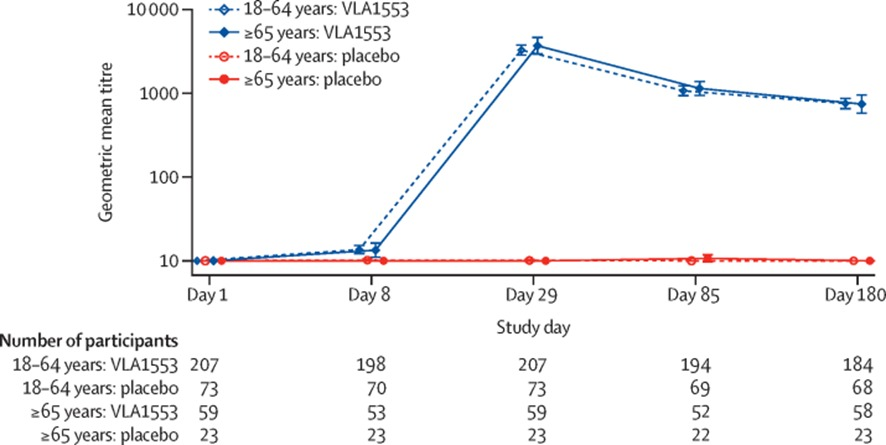
\includegraphics{img/placebo.jpeg}
\caption{resultados}
\end{figure}

\section{Validación externa e
interna}\label{validaciuxf3n-externa-e-interna}

Este estudio tuvo varias limitaciones. Primero, el estudio no se realizó
en una región endémica, por lo que se desconoce el efecto de la
inmunidad preexistente sobre la inmunogenicidad de VLA1553, así como el
perfil completo de seguridad en esta población. Segundo, la vacuna se
basa en una plataforma de virus vivo atenuado y, por tanto,
probablemente no sea utilizable en personas con inmunosupresión severa;
cualquier uso durante el embarazo deberá sopesar los riesgos graves para
los recién nacidos por la transmisión perinatal del chikunguña frente a
la práctica general de evitar o contraindicar las vacunas de virus vivo
atenuado durante el embarazo. Tanto las personas embarazadas como las
gravemente inmunocomprometidas fueron excluidas del ensayo como medida
de precaución. Tercero, la inmunogenicidad se determinó en un
subconjunto pequeño de participantes. Sin embargo, la población por
protocolo analizada para los desenlaces de inmunogenicidad fue
representativa de toda la población del estudio al comparar los datos
demográficos. Cuarto, para ser altamente eficaz en el control de una
enfermedad endémica, una vacuna contra el chikunguña también debe
administrarse a niños

El estudio tiene validez interna sólida porque cumple con las siguientes
consideraciones que deben tener los ensayos clínicos:

\begin{itemize}
\item
  Correcta aleatorización
\item
  Enmascaramiento (en este caso doble ciego)
\item
  Cumple con las buenas prácticas médicas
\item
  Los pacientes firman el consentimiento informado
\item
  Las definiciones de los eventos están bien explícitas
\item
  Existe un comité de ética
\end{itemize}

Pero, por lo mencionado anteriormente la validez externa es criticable,
dado que los resultados son aplicables a poblaciones sanas. Se necesitan
más datos en contextos endémicos y grupos vulnerables. Para una
evaluación definitiva, serían ideales estudios de fase 4 en condiciones
reales.

\section{Propuesta nuevo ensayo}\label{propuesta-nuevo-ensayo}

\subsection{Cálculo del tamaño de
muestra}\label{cuxe1lculo-del-tamauxf1o-de-muestra}

Se definen a continuación los valores del artículo:

\begin{itemize}
\item
  Nivel de significación: \(\alpha=0.05\)
\item
  Proporción de seroprotección en el grupo tratado con la vacuna:
  \(p_{tratamiento}=0.7\)
\item
  Tasa de abandono: \(R_0=0.1\)
\end{itemize}

Teniendo en cuenta estos valores se calcula el tamaño de muestra para el
grupo placebo para distintos valores de la proporción de seroprotección
en el grupo placebo y distintas potencias:

\begin{verbatim}
## Warning: Using `size` aesthetic for lines was deprecated in ggplot2 3.4.0.
## i Please use `linewidth` instead.
## This warning is displayed once every 8 hours.
## Call `lifecycle::last_lifecycle_warnings()` to see where this warning was
## generated.
\end{verbatim}

\includegraphics{reporte2_files/figure-latex/unnamed-chunk-2-1.pdf}

Seleccionamos una potencia del 90\% y una proporción para el grupo
placebo de 0.4. Con la combinación seleccionada obtenemos un tamaño de
muestra de \(58\) placebos y \(58 . 3 = 174\) tratamientos. En total
tenemos \(232\) pacientes para reclutar.

Si bien en el ensayo clínico plantea más análisis y deberíamos calcular
el temaño de muestra también para los otros, no tenemos los datos
suficientes para hacerlo. Además el objetivo principal del estudio es el
análisis de la seroprotección por lo que decidimos presentar los tamaños
de muestra solo para este propósito.

\subsection{Aleatorización}\label{aleatorizaciuxf3n}

\begin{Shaded}
\begin{Highlighting}[]
\FunctionTok{library}\NormalTok{(blockrand)}
\FunctionTok{library}\NormalTok{(randomizeR)}
\end{Highlighting}
\end{Shaded}

\begin{verbatim}
## Loading required package: plotrix
\end{verbatim}

\begin{verbatim}
## Loading required package: survival
\end{verbatim}

\begin{verbatim}
## Loading required package: mvtnorm
\end{verbatim}

\begin{Shaded}
\begin{Highlighting}[]
\FunctionTok{library}\NormalTok{(writexl)}
\NormalTok{imprimir\_excel}\OtherTok{=} \ConstantTok{FALSE}
\FunctionTok{set.seed}\NormalTok{(}\DecValTok{1889}\NormalTok{)}

\NormalTok{generar\_aleatorizacion\_estratificada }\OtherTok{\textless{}{-}} \ControlFlowTok{function}\NormalTok{(n\_placebo, n\_tratamiento, estratos, tratamientos, }\AttributeTok{n\_centros =} \DecValTok{1}\NormalTok{) \{}
\NormalTok{  n\_total\_por\_estrato }\OtherTok{\textless{}{-}}\NormalTok{ n\_placebo }\SpecialCharTok{+}\NormalTok{ n\_tratamiento}
\NormalTok{  resultados\_conteo }\OtherTok{\textless{}{-}} \FunctionTok{list}\NormalTok{()}
\NormalTok{  secuencias\_por\_estrato }\OtherTok{\textless{}{-}} \FunctionTok{list}\NormalTok{()}

  \ControlFlowTok{for}\NormalTok{ (estrato }\ControlFlowTok{in}\NormalTok{ estratos) \{}
\NormalTok{    conteo\_estrato }\OtherTok{\textless{}{-}} \FunctionTok{data.frame}\NormalTok{(}
      \AttributeTok{Estrato =}\NormalTok{ estrato,}
      \AttributeTok{Placebo =} \DecValTok{0}\NormalTok{,}
      \AttributeTok{Tratamiento =} \DecValTok{0}
\NormalTok{    )}
\NormalTok{    secuencia\_lista\_completa }\OtherTok{\textless{}{-}} \FunctionTok{character}\NormalTok{(}\DecValTok{0}\NormalTok{)}

    \ControlFlowTok{for}\NormalTok{ (i }\ControlFlowTok{in} \DecValTok{1}\SpecialCharTok{:}\NormalTok{n\_centros) \{}
      \CommentTok{\# Definir los parámetros para la aleatorización por bloques}
\NormalTok{      par\_adaptado }\OtherTok{\textless{}{-}} \FunctionTok{rpbrPar}\NormalTok{(}
        \AttributeTok{N =}\NormalTok{ n\_total\_por\_estrato,}
        \AttributeTok{rb =} \FunctionTok{c}\NormalTok{(}\DecValTok{4}\NormalTok{),}
        \AttributeTok{K =} \FunctionTok{length}\NormalTok{(tratamientos),}
        \AttributeTok{ratio =} \FunctionTok{c}\NormalTok{(}\DecValTok{1}\NormalTok{, }\DecValTok{3}\NormalTok{),}
        \AttributeTok{groups =}\NormalTok{ tratamientos,}
        \AttributeTok{filledBlock =} \ConstantTok{FALSE}
\NormalTok{      )}

      \CommentTok{\# Generar la secuencia de aleatorización}
      \FunctionTok{set.seed}\NormalTok{(}\DecValTok{2850} \SpecialCharTok{+}\NormalTok{ i }\SpecialCharTok{+} \FunctionTok{which}\NormalTok{(estratos }\SpecialCharTok{==}\NormalTok{ estrato) }\SpecialCharTok{*} \DecValTok{10}\NormalTok{)}
\NormalTok{      secuencia\_objeto }\OtherTok{\textless{}{-}} \FunctionTok{genSeq}\NormalTok{(par\_adaptado, }\DecValTok{1}\NormalTok{)}
\NormalTok{      secuencia\_lista }\OtherTok{\textless{}{-}} \FunctionTok{getRandList}\NormalTok{(secuencia\_objeto)}
\NormalTok{      secuencia\_lista\_completa }\OtherTok{\textless{}{-}} \FunctionTok{c}\NormalTok{(secuencia\_lista\_completa, secuencia\_lista)}

      \CommentTok{\# Contar las ocurrencias de cada tratamiento}
\NormalTok{      conteo\_placebo }\OtherTok{\textless{}{-}} \FunctionTok{sum}\NormalTok{(secuencia\_lista }\SpecialCharTok{==} \StringTok{"Placebo"}\NormalTok{)}
\NormalTok{      conteo\_tratamiento }\OtherTok{\textless{}{-}} \FunctionTok{sum}\NormalTok{(secuencia\_lista }\SpecialCharTok{==} \StringTok{"Tratamiento"}\NormalTok{)}

      \CommentTok{\# Acumular los conteos por estrato}
\NormalTok{      conteo\_estrato}\SpecialCharTok{$}\NormalTok{Placebo }\OtherTok{\textless{}{-}}\NormalTok{ conteo\_estrato}\SpecialCharTok{$}\NormalTok{Placebo }\SpecialCharTok{+}\NormalTok{ conteo\_placebo}
\NormalTok{      conteo\_estrato}\SpecialCharTok{$}\NormalTok{Tratamiento }\OtherTok{\textless{}{-}}\NormalTok{ conteo\_estrato}\SpecialCharTok{$}\NormalTok{Tratamiento }\SpecialCharTok{+}\NormalTok{ conteo\_tratamiento}
\NormalTok{    \}}
\NormalTok{    resultados\_conteo[[estrato]] }\OtherTok{\textless{}{-}}\NormalTok{ conteo\_estrato}

    \CommentTok{\# Crear el data frame de la secuencia para este estrato}
\NormalTok{    secuencia\_df\_estrato }\OtherTok{\textless{}{-}} \FunctionTok{data.frame}\NormalTok{(}\AttributeTok{Secuencia =}\NormalTok{ secuencia\_lista\_completa)}
    \FunctionTok{colnames}\NormalTok{(secuencia\_df\_estrato) }\OtherTok{\textless{}{-}} \FunctionTok{paste0}\NormalTok{(estrato, }\StringTok{"{-}"}\NormalTok{, }\DecValTok{1}\SpecialCharTok{:}\FunctionTok{ncol}\NormalTok{(secuencia\_df\_estrato)) }\CommentTok{\# Esto no es correcto para la estructura deseada}

    \CommentTok{\# La estructura correcta sería una fila por estrato con la secuencia como valores}
\NormalTok{    secuencias\_por\_estrato[[estrato]] }\OtherTok{\textless{}{-}} \FunctionTok{data.frame}\NormalTok{(}\FunctionTok{t}\NormalTok{(secuencia\_lista\_completa))}
    \FunctionTok{colnames}\NormalTok{(secuencias\_por\_estrato[[estrato]]) }\OtherTok{\textless{}{-}} \FunctionTok{paste0}\NormalTok{(}\StringTok{"Paciente"}\NormalTok{, }\DecValTok{1}\SpecialCharTok{:}\FunctionTok{length}\NormalTok{(secuencia\_lista\_completa))}
\NormalTok{  \}}

  \CommentTok{\# Combinar los resultados del conteo}
\NormalTok{  tabla\_distribucion }\OtherTok{\textless{}{-}} \FunctionTok{do.call}\NormalTok{(rbind, resultados\_conteo)}

  \CommentTok{\# Combinar las secuencias por estrato en un solo data frame}
\NormalTok{  secuencia\_aleatorizacion\_final }\OtherTok{\textless{}{-}} \FunctionTok{do.call}\NormalTok{(rbind, secuencias\_por\_estrato)}
\NormalTok{  secuencia\_aleatorizacion\_final}\SpecialCharTok{$}\NormalTok{Estrato }\OtherTok{\textless{}{-}} \FunctionTok{names}\NormalTok{(secuencias\_por\_estrato) }\CommentTok{\# Añadir la columna de estrato}

  \CommentTok{\# Reorganizar las columnas para que el estrato sea la primera}
\NormalTok{  secuencia\_aleatorizacion\_final }\OtherTok{\textless{}{-}}\NormalTok{ secuencia\_aleatorizacion\_final[, }\FunctionTok{c}\NormalTok{(}\StringTok{"Estrato"}\NormalTok{, }\FunctionTok{setdiff}\NormalTok{(}\FunctionTok{names}\NormalTok{(secuencia\_aleatorizacion\_final), }\StringTok{"Estrato"}\NormalTok{))]}


  \CommentTok{\# Devolver una lista con la tabla y la secuencia}
  \FunctionTok{return}\NormalTok{(}\FunctionTok{list}\NormalTok{(}\AttributeTok{tabla\_distribucion =}\NormalTok{ tabla\_distribucion, }\AttributeTok{secuencia\_aleatorizacion =}\NormalTok{ secuencia\_aleatorizacion\_final))}
\NormalTok{\}}
\end{Highlighting}
\end{Shaded}

\begin{Shaded}
\begin{Highlighting}[]
\DocumentationTok{\#\# Parámetros del estudio}
\NormalTok{n\_placebo }\OtherTok{\textless{}{-}} \DecValTok{58}         \CommentTok{\# Tamaño grupo placebo}
\NormalTok{n\_tratamiento }\OtherTok{\textless{}{-}} \DecValTok{58} \SpecialCharTok{*} \DecValTok{3} \CommentTok{\# Tamaño grupo tratamiento (3:1)}
\NormalTok{n\_total }\OtherTok{\textless{}{-}}\NormalTok{ n\_placebo }\SpecialCharTok{+}\NormalTok{ n\_tratamiento}
\NormalTok{estratos }\OtherTok{\textless{}{-}} \FunctionTok{c}\NormalTok{(}\StringTok{"18{-}64"}\NormalTok{, }\StringTok{"+65"}\NormalTok{)  }\CommentTok{\# Dos estratos de edad}
\NormalTok{tratamientos }\OtherTok{\textless{}{-}} \FunctionTok{c}\NormalTok{(}\StringTok{"Placebo"}\NormalTok{, }\StringTok{"Tratamiento"}\NormalTok{)}
\NormalTok{n\_centros }\OtherTok{\textless{}{-}} \DecValTok{1}

\CommentTok{\# Ejecutar la función}
\NormalTok{resultados\_aleatorizacion }\OtherTok{\textless{}{-}} \FunctionTok{generar\_aleatorizacion\_estratificada}\NormalTok{(}
  \AttributeTok{n\_placebo =}\NormalTok{ n\_placebo,}
  \AttributeTok{n\_tratamiento =}\NormalTok{ n\_tratamiento,}
  \AttributeTok{estratos =}\NormalTok{ estratos,}
  \AttributeTok{tratamientos =}\NormalTok{ tratamientos,}
  \AttributeTok{n\_centros =}\NormalTok{ n\_centros}
\NormalTok{)}

\CommentTok{\# \# Imprimir la tabla de distribución}
\CommentTok{\# print("Tabla de Distribución por Tratamiento y Grupo Etario:")}
\CommentTok{\# print(resultados\_aleatorizacion$tabla\_distribucion)}
\CommentTok{\# }
\CommentTok{\# \# Imprimir la secuencia de aleatorización}
\CommentTok{\# print("\textbackslash{}nSecuencia de Aleatorización Completa:")}
\CommentTok{\# print(resultados\_aleatorizacion$secuencia\_aleatorizacion)}

\ControlFlowTok{if}\NormalTok{(imprimir\_excel)}
  \CommentTok{\# Opcional: Guardar la secuencia en un archivo Excel}
  \FunctionTok{write\_xlsx}\NormalTok{(resultados\_aleatorizacion}\SpecialCharTok{$}\NormalTok{secuencia\_aleatorizacion, }
             \AttributeTok{path =} \StringTok{"secuencia\_aleatorizacion.xlsx"}\NormalTok{)}

  \CommentTok{\# Opcional: Guardar la tabla de distribución en un archivo Excel}
  \FunctionTok{write\_xlsx}\NormalTok{(resultados\_aleatorizacion}\SpecialCharTok{$}\NormalTok{tabla\_distribucion, }
             \AttributeTok{path =} \StringTok{"tabla\_distribucion.xlsx"}\NormalTok{)}
\end{Highlighting}
\end{Shaded}

\subsection{Análisis estadístico}\label{anuxe1lisis-estaduxedstico}

Ya que el tamaño de muestra es lo suficientemente grande, se puede
realizar la aproximación Normal de la Binomial para realizar un test Z.
En este se desea comparar dos proporciones, p1 y p2 , observadas en dos
grupos distintos de tamaños n1 y n2 , respectivamente.

\begin{itemize}
\item
  \(H_0)\) \(p_{tratamiento}=p_{placebo}\)
\item
  \(H_1)\) \(p_{tratamiento} > p_{placebo}\)
\end{itemize}

\textbf{Estadística:}

\[
Z = \frac{p_1 - p_2}{EED} = \frac{p_1 - p_2}{\sqrt{\frac{p_1 (1 - p_1)}{n_1} + \frac{p_2 (1 - p_2)}{n_2}}}
\]

El estadístico Z sigue una distribución Normal (0, 1).

\textbf{Regla de decisión:}

Rechazar \(H_0\) si \(p-value < \alpha\)

La ventaja de este test es que se puede calcular un intervalo de
confianza \((p1-p2 ) Z* EED\) donde EED corresponde al error estándar de
la diferencia de proporciones como se calcula en la fórmula anterior.

\end{document}
